% !TEX root = lectures.tex
%!TEX encoding = UTF-8 Unicode
%% !TEX root =  lectures.tex
\documentclass[12pt]{article}
\usepackage{graphicx}
\usepackage[
	pdfencoding=auto,%
	pdftitle={PHY 321, Classical Mechanics I, Lecture Notes},%
	pdfauthor={Scott Pratt},%
	pdfstartview=FitV,%
	colorlinks=true,%
	linkcolor=blue,%
	citecolor=black, %
	urlcolor=blue]{hyperref}
%\usepackage{pdfsync}
\usepackage{amssymb}
\usepackage{amsmath}
\usepackage{bm}
\usepackage{bbold}
\numberwithin{equation}{section} 
\numberwithin{figure}{section} 
\usepackage[small,bf]{caption}

\usepackage{fontspec}
\usepackage{textcomp}
\usepackage{graphicx}
\usepackage{color}
\usepackage{fancyhdr}
\usepackage{bm}

\newcounter{examplecounter}
\setcounter{examplecounter}{0}
\newcommand{\example}{
\stepcounter{examplecounter}{\nopagebreak\noindent\rule{\textwidth}{1pt}\nopagebreak\\ \bf Example \nopagebreak \arabic{section}.\arabic{examplecounter}:\\ \nopagebreak}}

\newcommand{\exampleend}{
\begin{samepage}
\nopagebreak\noindent\rule{\textwidth}{1pt}
\end{samepage}}

%\usepackage[T1]{fontenc}
%\renewcommand*{\sfdefault}{Berenis}
%\renewcommand*{\rmdefault}{Berenis}
%\renewcommand*{\sfdefault}{phv} % helvetica
%\renewcommand*{\sfdefault}{ppl} % palatino
%\renewcommand*{\rmdefault}{ppl}
%\renewcommand*{\sfdefault}{Bookman}
%\renewcommand*{\rmdefault}{Bookman}

\defaultfontfeatures{Scale=MatchLowercase}
%\setmainfont[Mapping=tex-text,SmallCapsFont={CalifornianFB Expert}]{CalifornianFB}
%\setmainfont[Mapping=tex-text]{Minion Pro}
\setmainfont[Mapping=tex-text]{Palatino Bold}
\setmonofont[Mapping=tex-text]{Courier New Bold}
%\setsansfont[Mapping=tex-text]{Myriad Pro}
%\usepackage{xltxtra}
%\setromanfont{Palatino}
\setromanfont{Palatino Bold}


%\pagestyle{empty}
\textwidth 7.0in
\hoffset -0.8in
\textheight 9.4in
\voffset -1in

\pagestyle{fancy}             % page layout
\newcommand{\TheShortTitle}{}
\newcommand{\ShortTitle}[1]{\renewcommand{\TheShortTitle}{#1}}
\fancyhead[LO,RE]{\slshape \TheShortTitle}
\fancyhead[LE,RO]{\slshape \leftmark}

\usepackage{colortbl}
\newcommand{\cc}[1]{\cellcolor{#1}}
\definecolor{lightred}{rgb}{1,0.5,0.6}
\definecolor{lightblue}{rgb}{0.6,0.8,1.0}

\usepackage{comment}
\parskip 4pt
\parindent 0pt

%\newcommand{\bm}{\boldmath}
\boldmath

% for the banner across the tops of pages 2-
\ShortTitle{PHY 831}

\ShortTitle{PHY 321 Lecture Notes}

\section{Lagrangians and the Calculus of Variations}
\label{sec:lagrangians}
\bigskip

\subsection{Calculus of Variations and the Euler-Lagrange Equation}

The usual minimization problem one faces involves taking a function
$J(y)$, then finding the single value $y$ for which $J$ is either a
maximum or minimum. In multivariate calculus one also learns to solve
problems where you minimize for multiple variables, $J(y_1,y_2,\cdots
y_n)$, and finding the point $(y_1\cdots y_n)$ in $n-$dimensional
space that maximizes or minimizes the function. Here, we consider what
seems to be a much more ambitious problem. Imagine you have a function
$J(y(x),y'(x);x)$, and you wish to find the extrema for an infinite
number of values of $y$, i.e. $y$ at each point $x$. The function $J$
will not only depend on $y$ at each point $x$, but also on the slope
at each point, plus an additional dependence on $x$. Note we are NOT
finding an optimum value of $x$, we are finding the set of optimum
values of $y$ at each point $x$, or equivalently, finding the function
$y(x)$.

One treats the function $y(x)$ as being unknown while minimizing
\[
J=\int_{x_1}^{x_2}dx~f\{y(x),y'(x);x\}.
\]
Thus, we are minimizing $J$ with respect to an infinite number of
values of $y(x_i)$ at points $x_i$. As an additional criteria, we will
assume that $y(x_1)$ and $y(x_2)$ are fixed, and that that we will
only consider variations of $y$ between the boundaries. The dependence
on the derivative, $y'=dy/dx$, is crucial because otherwise the
solution would involve simply finding the one value of $y$ that
minimized $f$, and $y(x)$ would equal a constant if there were no
explicit $x$ dependence. Furthermore, $y$ wouldn't need to be
continuous at the boundary.

The Euler equation is a differential equation for $y(x)$, that when
solved, provides the required solution. For an extrema
\begin{eqnarray}
\delta J&=&\int_{x_1}^{x_2}dx~\left\{ \frac{\partial f}{\partial
  y}\delta y(x)+\frac{\partial f}{\partial y'}\delta y'(x)\right\}=0.
\end{eqnarray}
For ANY small $\delta y(x)$ at any point $x$, the change should be
zero if one is at an optimum function $y(x)$. Integrating the second
term by parts,
\begin{eqnarray}
\delta J&=&\int_{x_1}^{x_2}dx~\left\{ \frac{\partial f}{\partial
  y}-\frac{d}{dx}\left(\frac{\partial f}{\partial
  y'}\right)\right\}\delta y(x)\\ \nonumber &&+\left.\frac{\partial
  f}{\partial y'}\delta y\right|_{x_2}-\left.\frac{\partial
  f}{\partial y'}\delta y\right|_{x_1}\\ \nonumber &=&0.
\end{eqnarray}
Because $y$ is not allowed to vary at the endpoints, $\delta
y(x_1)=\delta y(x_2)=0$, so the middle line can be ignored.  Also,
this relation must hold for ANY $\delta y$, so one can write the Euler
equations (or sometimes called the Euler Lagrange equations)
\begin{equation}
\label{eq:el}
\frac{\partial f}{\partial y}=\frac{d}{dx}\frac{\partial f}{\partial
  y'}.
\end{equation}
This will yield a differential equations for $y$. Combined with the
boundary conditions,
\begin{equation}
y(x_1)=y_1, ~~~y(x_2)=y_2,
\end{equation}
one can now solve the differential equations for $y$. Because $f$ is
only a function of $f'$, not $f''$ or $f'''$, the $d/dx$ in Euler
Lagrange equation can lead to terms involving $f''$, but not
$f'''$. Thus, the equation will be a second-order differential
equation (not a linear equation usually), and the two boundary
conditions are sufficient to determine the entire equation.

\example\label{ex:brachiostone}\noindent Consider a particle
constrained to move along a path (like a bead moving without friction
on a wire) and you need to design a path from $x=y=0$ to some final
point $x_f,y_f$. Assume there is a constant force in the $x$
direction, $F_x=mg$. Design the path so that the time the bead travels
is a minimum.

{\bf Solution:} The net time is
\[
T=\int \frac{d\ell}{v}=\int_0^{x_f}
dx~\frac{\sqrt{1+y'^2}}{\sqrt{2gx}}={\rm minimum}.
\]
Here we made use of the fact that $d\ell=\sqrt{dx^2+dy^2}$ and that
the velocity is determined by $KE=mv^2/2=mgx$. The Euler equations can
be applied if you first define the function as
\begin{eqnarray*}
f(y,y';x)&=&\frac{\sqrt{1+y'^2}}{\sqrt{x}}.
\end{eqnarray*}
The equations are then
\begin{eqnarray*}
\frac{d}{dx}\frac{\partial f}{\partial y'}&=&0.
\end{eqnarray*}
The simplification ensued from $f$ not having any dependence on
$y$. This yields the differential equation
\begin{eqnarray}
\frac{y'}{x^{1/2}(1+y'^2)^{1/2}}&=&(2a)^{-1/2},
\end{eqnarray}
because $\partial f/\partial y'$ must be a constant, which with some
foresight we label $(2a)^{-1/2}$. One can now solve for $y'$,
\begin{eqnarray*}
(y')^2&=&2ax(1+y'^2)\\ \nonumber
  y'&=&\sqrt{\frac{x}{2a-x}},\\ \nonumber y(x)&=&\int_0^x
  dx'~\frac{\sqrt{x'}dx'}{\sqrt{2a-x'}}=\int_0^x
  dx'~\frac{x'dx'}{\sqrt{2ax'-x'^2}}\\ \nonumber
  &=&\frac{1}{2}\int_0^x\frac{(2x'-2a)dx'}{(2ax'-x'^2)^{1/2}}+a\int_0^x\frac{dx'}{\sqrt{2ax'-x'^2}}\\ \nonumber
  &=&\frac{-1}{2}\int_0^{2ax-x^2}\frac{du}{\sqrt{u}}+a\int_0^x\frac{dx'}{\sqrt{a^2-(x'-a)^2}}\\ &=&-\sqrt{2ax-x^2}+a\cos^{-1}(1-x/a).
\end{eqnarray*}
This turns out to be the equation for a {\it cycloid} or a {\it
  brachiostone}. If you rolled a wheel of radius $a$ down the $y$ axis
and followed a point on the rim, it would trace out a cycloid. Here,
the constant $a$ must be chosen to match the boundary condition,
$y_2=y(x_2)$. You can see the textbook for more details, plus you get
a chance to work with cycloids in the exercises at the end of this
chapter.

\exampleend

\subsection{Auxiliary Constraints}

Sometimes an auxiliary constraint is added to the problem (beyond
fixing the end poits $y_1$ and $y_2$). Just ahead, we will work on the
example of a hanging chain. The shape of the curve minimizes the
potential energy, under the constraint of a fixed length of
chain. Before presenting such an example we first review the method of
Lagrange multipliers as a method for finding minima or maxima under
constraints.

Imagine a function $f(x_1,x_2\cdots x_n)$ for which you wish to find
the minima. Additionally, you are given a constraint
\begin{eqnarray}
C(x_1\cdots x_n)=0
\end{eqnarray}
The usual condition for a a minimum is
\begin{eqnarray}
\frac{\partial f}{\partial x_i}=0{\rm ,~~or~}\nabla f=0.
\end{eqnarray}
which would be $n$ equations for the $n$ variables. The gradient of a
scalar is a vector, so you should think of $\nabla$ as
$\vec{\nabla}$. However, the solution will likely not satisfy the
constraint, i.e. the point at which $f(x_1\cdots x_n)$ has an extrema,
may not be a point where $C(x_1\cdots x_n)=0$.

A necessary condition for the solution is that
\begin{equation}
\nabla f\cdot\vec{\epsilon}=0,
\end{equation}
for any infinitesimal vector $\vec{\epsilon}$ if $\vec{\epsilon}$
satisfies the condition
\begin{equation}
\delta C=\nabla C\cdot\vec{\epsilon}=0.
\end{equation}
That is to say if I take a small step in a direction that doesn't
change the constraint, then $f$ must not change if it is an
extrema. Not changing the constraint implies the step is orthogonal to
$\nabla C$. As there are $n$ dimensions of $x$, the vector $\nabla C$
defines one direction, and $\vec{\epsilon}$ can be in any of the $n-1$
directions orthogonal to $\nabla C$. If $\nabla
f\cdot\vec{\epsilon}=0$ for ANY of the $n-1$ directions of
$\vec{\epsilon}$ orthogonal to $\nabla C$, then
\begin{equation}
\nabla f ~||~ \nabla C.
\end{equation}
Because the two vectors are parallel you can say there must exist some
constant $\lambda$ such that
\begin{equation}
\label{eq:lagrangemultiplier}
\nabla(f-\lambda C)=0.
\end{equation}
Here, $\lambda$ is known as a Lagrange multiplier. Satisfying
Eq. (\ref{eq:lagrangemultiplier}) is a necessary, but not a sufficient
condition. One could add a constant to the constraint and the gradient
would not change. One must find the correct value of $\lambda$ that
satisfies the constraint $C=0$, rather than $C=$ some other
constant. The strategy is then to solve
Eq. (\ref{eq:lagrangemultiplier}) then adjust $\lambda$ until one
finds the $x_1\cdots x_n$ that gives $C(x_1\cdots x_n)=0$.

The method of Lagrange multipliers is counter-intuitive to one's
intuition to use the constraint to reduce the dimensionality of the
problem. Normally, minimizing a function of $n$ variables, leads to
$n$ equations and $n$ unknowns. A constraint could be used, by
substitution, to replace the $n$ variables with $n-1$
variables. Instead, we add an unknown parameter, $\lambda$, and change
the equation to $n+1$ equations with $n+1$ unknowns, with the extra
unknown being the Lagrange multiplier $\lambda$. Often, it is rather
easy to solve for $x_1\cdots x_n$. Then one is left with the usually
difficult problem of finding $\lambda$, often requiring the solution
of a transcendental equation.

\example As an example of using Lagrange multipliers for a standard
optimization formula we attempt to maximize the following function,
\[
F(x_1\cdots x_n)=-\sum_{i=1}^n x_i\ln(x_i),
\]
with respect to the $n$ variables $x_i$. With no constraints, each
$x_i$ would maximize the function for
\begin{eqnarray*}
\frac{d}{dx_j}~\left[-\sum_i
  x_i\ln(x_i)\right]&=&0\\ -\ln(x_j)-1&=&0,~~~~x_j=e^{-1}.
\end{eqnarray*}
Now, we repeat the problem but with two constraints,
\[
\sum_ix_i=1~,~~~~\sum_ix_i\epsilon_i=E.
\]
Here, $\epsilon_i$ and $E$ are fixed constants. We go forward by
finding the extrema for
\begin{eqnarray*}
G(x_1\cdots x_n)&=&F-\alpha\sum_i x_i-\beta\sum_i\epsilon_ix_i =\sum_i
\left\{-x_i\ln(x_i)-\alpha x_i-\beta\epsilon_ix_i\right\}.
\end{eqnarray*}
There are two Lagrange multipliers, $\alpha$ and $\beta$,
corresponding to the two constraints. One then solves for the extrema
\begin{eqnarray*}
\frac{d}{dx_j}G&=&0\\ &=&-\ln(x_j)-1-\alpha-\beta\epsilon_j,\\ x_j&=&\exp\left\{-1-\alpha-\beta\epsilon_j\right\}.
\end{eqnarray*}
For any given $\alpha$ and $\beta$ this provides a solution for
constraining $\sum_i x_i$ and $\sum_i\epsilon_ix_i$ to some values,
just not the values of unity and $E$ that you wish. One would then
have to search for the correct values by adjusting $\alpha$ and
$\beta$ until the constraint are actually matched by solving a
transcendental equation. Although this can be complicated, it is
certainly less expensive than searching over all $N$ values of
$x_i$. This particular example corresponds to maximizing the entropy
for a system, $S=-\sum_i x_i\ln(x_i)$, where $x_i$ is the probability
of the system being in a particular discrete level $i$ that has energy
$\epsilon_i$. One wishes to maximize the entropy subject to the
constraints that the probabilities sum to unity and the average energy
has some given value. The result that $x_i\sim e^{-\beta\epsilon_i}$
demonstrates the origin of the Boltzmann factor, with the inverse
temperature $\beta=1/T$.

\exampleend

Lagrange multipliers also assist with the Euler-Lagrange equation. If
one breaks an interval $x_1<x<x_2$ into a large number
$n\rightarrow\infty$ points separated by $dx$, the Euler-Lagrange
equation involves finding the $n$ values $y_i$ at each point so that
$\sum_i dx f\left\{y_i,y'_i=(y_{i+1}-y_{i-1})/(2dx)\right\}$ is
maximized for some given function $f$. If an additional auxiliary
constraint is added, also some function of the $n$ values $y_i$, one
can use the method of Lagrange multipliers. In the constraint can also
be written as some function of $C(y_i,y'_i)$, then one simply adds a
term $\lambda C(y,y')$ to the function $f$ and uses the Euler-Lagrange
equation to find the extrema of.
\begin{eqnarray}
J&=&\int_{x_1}^{x_2}dx~f\left\{y(x),y'(x),x\right\}-\lambda
C\left\{y(x),y'(x),x\right\},
\end{eqnarray}
the one difference being that
\begin{equation}
f\left\{y(x),y'(x),x\right\}\rightarrow
f\left\{y(x),y'(x),x\right\}-\lambda C\left\{y(x),y'(x),x\right\}
\end{equation}
in Eq. (\ref{eq:el}).

\example Consider a chain of length $L$ and mass per unit length
$\kappa$ that hangs from point $x=0,y=0$ to point $x_f,y_f$. The shape
must minimize the potential energy. Find general expressions for the
shape in terms of three constants which must be chosen to match
$y(0)=0, y(x_f)=y_f$ and the fixed length. Equivalently, one finds the
function $y(x)$ that provides an extrema for the integral,

{\bf Solution:} One must minimize
\[
\int d\ell~\kappa gy-\lambda\int d\ell= \int_0^{x_f}
dx~\sqrt{1+y'^2}\kappa gy-\lambda \int_0^{x_f} dx\sqrt{1+y'^2}.
\]
Here $\lambda$ is the Lagrange multiplier associated with constraining
the length of the chain. The constrained length $L$ appears nowhere in
the expression. Instead, one solves for form of the answer, then
adjusts $\lambda$ to give the correct length. For the purposes of the
Euler-Lagrange minimization one considers the function
\begin{eqnarray}
f(y,y';x)&=&\kappa gy\sqrt{1+y'^2}-\lambda\sqrt{1+y'^2}.
\end{eqnarray}
Because $\lambda$ is an unknown constant and because minimizing a
function multiplied by a constant is the same as minimizing the
function, we can equivlently minimize the integral using the function
\begin{eqnarray}
\tilde{f}(y,y';x)&=&y\sqrt{1+y'^2}-\tilde{\lambda}\sqrt{1+y'^2},\\ \nonumber
\tilde{\lambda}&\equiv&\frac{\lambda}{\kappa g}.
\end{eqnarray}
The Euler-Lagrange equations then become
\begin{eqnarray*}
\frac{d}{dx}\left\{
\frac{y'}{\sqrt{1+y'^2}}y-\tilde{\lambda}\frac{y'}{\sqrt{1+y'^2}}
\right\}&=&\sqrt{1+y'^2}.
\end{eqnarray*}
Here, we will guess at the form of the solution,
\begin{eqnarray*}
y'&=&\sinh[(x-x_0)/a],~~y=a\cosh[(x-x_0)/a]+y_0.
\end{eqnarray*}
Plugging into the Euler-Lagange equations,
\begin{eqnarray*}
\frac{d}{dx}\left\{(a\cosh[(x-x_0)/a]+y_0)\frac{\sinh[(x-x_0)/a]}{\cosh[(x-x_0)/a]}-\tilde{\lambda}\frac{\sinh[(x-x_0)/a]}{\cosh[(x-x_0)/a]}\right\}&=&\cosh[(x-x_0)/a],\\ \nonumber
\frac{d}{dx}\left\{(y_0-\tilde{\lambda})\tanh[(x-x_0)/a]\right\}=0.
\end{eqnarray*}
This solution works if $y_0=\tilde{\lambda}$. So the general form of
the solution is
\[
y=\tilde{\lambda}+a\cosh[(x-x_0)/a].
\]
One must find $\tilde{\lambda}$, $x_0$ and $a$ to satisfy three
conditions, $y(x=0)=0$, $y(x=x_f)=y_f$ and that the length is $L$. For
a hanging chain $a$ is positive. A solution with negative $a$ would
represent a maximum of the potential energy. A remarkable property of
the solution is that once you define the length and the end-point
positions $y_1$ and $y_2$, the solution does not depend on $\kappa$ or
$g$. Thus, the shape of the chain would be the same if you took it to
the moon. These solutions are known as {\it
  catenaries},\\ \href{http://en.wikipedia.org/wiki/Catenary}{http://en.wikipedia.org/wiki/Catenary}.

\exampleend

\subsection{Lagrangians}

Lagrangians represent a powerful method for solving problems that
would be nearly impossible by direct application of Newton's third
law, $\vec{F}=m\vec{a}$. The method works well for problems where a
system is well described by a few \textit{generalized coordinates}. A
generalized coordinate might be the angle describing the position of a
pendulum. This one angle takes the place of using $x$ and $y$ to
describe the position of the pendulum, then applying a clumsy
constraint.

The Lagrangian equations of motion can be derived from a principle of
least action, where the action $S$ is defined as
\begin{equation}
S=\int dt~ L(q,\dot{q},t),
\end{equation}
where $q$ is some coordinate that describes the orientation of a
system and the Lagrangian $L$ is defined as
\begin{equation}
L=T-U,
\end{equation}
the difference of the kinetic and potential energies. Minimizing the
action through the Euler-Lagrange equations gives the Lagrangian
equations of motion,
\begin{equation}
\frac{d}{dt}\frac{\partial L}{\partial \dot{q}}=\frac{\partial
  L}{\partial q}.
\end{equation}
We begin with two simple examples, neither of which gains from the
Lagrangian approach.

\example Consider a particle of mass $m$ connected to a spring with
stiffness $k$. Derive the Lagrangian equations of motion.\\ {\bf
  Solution:}
\begin{eqnarray*}
L&=&\frac{1}{2}m\dot{x}^2-\frac{1}{2}kx^2,\\ \frac{d}{dt}\frac{\partial
  L}{\partial \dot{x}}&=&\frac{\partial L}{\partial
  x},\\ m\ddot{x}&=&-kx.
\end{eqnarray*}

\example Derive the Lagrangian equations of motion for a pendulum of
mass $m$ and length $\ell$.
\begin{eqnarray*}
L&=&\frac{m}{2}\ell^2\dot{\theta}^2-mg\ell(1-\cos\theta),\\ \frac{d}{dt}\frac{\partial
  L}{\partial \dot{\theta}}&=&\frac{\partial L}{\partial
  \theta},\\ m\ell^2\ddot{\theta}&=&-mg\ell\sin\theta,\\ \ddot{\theta}&=&-\frac{g}{\ell}\sin\theta,\\ \ddot{\theta}&\approx&-\frac{g}{\ell}\theta.
\end{eqnarray*}
\exampleend

\subsection{Proving Lagrange's Equations of Motion from Newton's Laws}

Lagrange's equations of motion can only be applied for the following
conditions:
\begin{enumerate}
\item The potential energy is a function of the generalized
  coordinates $q_i$, but not of $\dot{q}_i$.
\item The relation between the original coordinates $x,y,z\cdots$ and
  the generalized coordinates does not depend on $\dot{q}_i$,
  e.g. $x(q,t)$ not $x(q,\dot{q},t)$.
\item Any constraints used to reduce the number of degrees of freedom
  are functions of $\vec{q}$, but not of $\dot{\vec{q}}$.
\item The motion is not dissipative (no damping or friction).
\end{enumerate}
Going forward with the proof, consider $x_i(q_1,q_2\cdots,t)$ and look
at the l.h.s. of Lagrange's equations of motion.
\begin{eqnarray}
\label{eq:lagrangederivation1}
\frac{\partial T}{\partial\dot{q}_j}&=&\sum_i\frac{\partial
  T}{\partial\dot{x}_i}\frac{\partial\dot{x}_i}{\partial\dot{q_j}}
+\sum_i\frac{\partial T}{\partial x_i}\frac{\partial
  x_i}{\partial\dot{q_j}}\\ \nonumber &=&\sum_i
m\dot{x}_i\frac{\partial \dot{x}_i}{\partial\dot{q_j}}\\ \nonumber
&=&\sum_i m\dot{x}_i\frac{(\delta x_i/\delta t)|_{{\rm fixed~}q_{j'\ne
      j}}}{\delta q_j/\delta t}\\ \nonumber
&=&\sum_im\dot{x}_i\frac{\delta{x}_i|_{{\rm fixed~}q_{j'\ne
      j}}}{\delta q_j}\\ \nonumber &=&\sum_i m\dot{x}_i\frac{\partial
  x_i}{\partial q_j}.
\end{eqnarray}
In the first line we used the fact that $T$ does not depend on
$x$. Continuing with taking the derivative of $U$,
\begin{eqnarray}
-\frac{\partial U}{\partial\dot{q}_j}&=&-\sum_i\frac{\partial
  U}{\partial x_i}\frac{\partial x_i}{\partial\dot{q}_j}=0.
\end{eqnarray}
In the first line above we used the fact that $U$ does not depend on
$\dot{x}$ then we used the second condition that $x$ does not depend
on $\dot{q}$. Adding the two pieces together, then taking the
derivative w.r.t. time,
\begin{eqnarray}
\nonumber
\frac{d}{dt}\frac{\partial}{\partial\dot{q}}(T-U)&=&\sum_im\ddot{x}_i\frac{\partial
  x_i}{\partial q_j} +\sum_i
m\dot{x}_i\frac{\partial\dot{x}_i}{\partial q_j}.
\end{eqnarray}

Now, we consider the r.h.s. of Lagrange's equations. Because the
kinetic energy depends only on $\dot{x}$ and not $x$, and because the
potential depends on $x$ but not $\dot{x}$,
\begin{eqnarray}
\label{eq:lagrangederivation2}
\frac{\partial}{\partial q_j}(T-U)&=&\sum_i\frac{\partial
  T}{\partial\dot{x}_i}\frac{\partial\dot{x_i}}{\partial q_j}
-\sum_i\frac{\partial U}{\partial x_i}\frac{\partial x_i}{\partial
  q_j}\\ \nonumber &=&\sum_i
m\dot{x}_i\frac{\partial\dot{x_i}}{\partial q_j} -\sum_i\frac{\partial
  U}{\partial x_i}\frac{\partial x_i}{\partial q_j}
\end{eqnarray}
Using the fact that $m\ddot{x}_i=-(\partial/\partial x_i)U$, one can
see that the bottom expressions in Eq.s (\ref{eq:lagrangederivation1})
and (\ref{eq:lagrangederivation2}) are identical,
\begin{equation}
\frac{d}{dt}\frac{\partial}{\partial\dot{q}_i}(T-U)=\frac{\partial}{\partial
  q_i}(T-U).
\end{equation}

\subsection{Lagrangian Examples}

Two examples are presented here. In the first, there are two
generalized coordinates, but the two equations of motion can be
reduced to one through conservation laws (angular momentum in this
case). In the second, there is a time-dependent constraint.

\example Consider a cone of half angle $\alpha$ standing on its tip at
the origin. The surface of the cone is defined as
\[
r=\sqrt{x^2+y^2}=z\tan \alpha.
\]
Find the equations of motion for a particle of mass $m$ moving along
the surface under the influence of a constant gravitational force,
$-mg\hat{z}$. For generalized coordinates use the azimuthal angle
$\phi$ and $r$.

{\bf Solution:}\\ The kinetic energy is
\begin{eqnarray*}
T&=&\frac{1}{2}mr^2\dot{\theta}^2+\frac{1}{2}m(\dot{r}^2+\dot{z}^2)\\ &=&\frac{1}{2}mr^2\dot{\theta}^2+\frac{1}{2}m\dot{r}^2\left(1+\cot^2\alpha\right)\\ &=&\frac{1}{2}mr^2\dot{\theta}^2+\frac{1}{2}m\dot{r}^2\csc^2\alpha.
\end{eqnarray*}
The potential energy is
\[
U=mgr\cot\alpha,
\]
so Lagrange's equations give
\begin{eqnarray*}
\frac{d}{dt}\left(mr^2\dot{\theta}\right)&=&0,\\ \frac{d}{dt}\left(m\csc^2\alpha
\dot{r}\right)&=&mr\dot{\theta}^2-mg\cot\alpha,\\ \ddot{r}&=&r\dot{\theta}^2\sin^2\alpha-g\cos\alpha\sin\alpha
\end{eqnarray*}
The first equation is a statement of the conservation of angular
momentum with $L=mr^2\dot{\theta}$, so the second equation can also be
expressed as
\[
\ddot{r}=\frac{L^2\sin^2\alpha}{m^2r^3}-g\sin\alpha\cos\alpha.
\]

\example A bead slides along a wire bent in the shape of a parabola,
\[
z=\frac{1}{2}kr^2,~~r^2=x^2+y^2.
\]
Also, the parabolic wire is rotating about the $z$ axis with angular
velocity $\omega$. Derive the equations of motion. Are there any
stable configurations?

{\bf Solution:}\\ Using the fact that
\[
\dot{z}=\dot{r}\frac{\partial z}{\partial r}=kr\dot{r},
\]
the kinetic and potential energies are
\begin{eqnarray*}
T&=&\frac{1}{2}m\left(\dot{r}^2+\dot{z}^2+r^2\omega^2\right)\\ &=&\frac{1}{2}m\left(\dot{r}^2+(kr\dot{r})^2+r^2\omega^2\right),\\ U&=&mgkr^2/2.
\end{eqnarray*}
The equations of motion are then
\begin{eqnarray*}
\frac{d}{dt}\left\{m\dot{r}(1+k^2r^2)\right\}&=&-mgkr+mk^2\dot{r}^2r+m\omega^2r,\\ \ddot{r}&=&\frac{-gkr+\omega^2r-k^2\dot{r}^2r}{1+k^2r^2}
\end{eqnarray*}
For a stable configuration, there needs to be a solution with
$\dot{r}=0$ and $\ddot{r}=0$. This can only happen at $r=0$, and then
for the acceleration to be inward for small deviations of $r$ one
needs to have $gk>\omega^2$. If $\omega^2>gk$ the bead will move
outward indefinitely.

\subsection{Small Vibrations and Normal Modes}

Two examples are provided for solving for normal modes. These are
solutions with multiple generalized coordinates, where the motion is
that of simple harmonic motion. However, the motion is only simple for
a particular set of coordinates $q_1$ and $q_2$,
\begin{eqnarray}
q_1&=&A\cos(\omega_1 t),\\ \nonumber q_2&=&B\cos(\omega_2 t),
\end{eqnarray}
while it is not necessarily simple in other coordinates. For example
if $x=q_1+q_2$, and $y=q_1-q_2$, the $x$ and $y$ motions will contain
mixtures of multiple frequencies. For many problems, or in the limit
of small vibrations about a minimum, there is some coordinate system
where the motion is simple. These are normal modes. Characterizing the
normal modes involves finding the frequencies, $\omega_i$, and the
coordinate system where the motion is simple for each coordinate. This
involves finding the direction, or the linear combination of $x_i$
that form the coordinates $q_i$ in which the motion is that of a
single oscillator in each coordinate.

For a first example, we consider a system of springs, where we write
the Lagrangian, then find the normal modes. For the second example, a
double pendulum is considered. In this case, one must first make a
small angle expansion before finding the modes. In principle, problems
could have the same number of normal modes a degrees of freedom. For
example, a system of 7 particles moving in three dimensions has 21
degrees of freedom. However, some of the degrees of freedom do not
have oscillatory behavior. For example, for a rigid body in free
space, the angles describing the orientation evolve, but do not
oscillate. Also, the center-of-mass coordinates of a system of
particles isolated from outside particles moves at constant
velocity. One can also describe these as normal modes, but acknowledge
that their characteristic frequency is zero, as there are no restoring
forces.

\example
\begin{figure}
\centerline{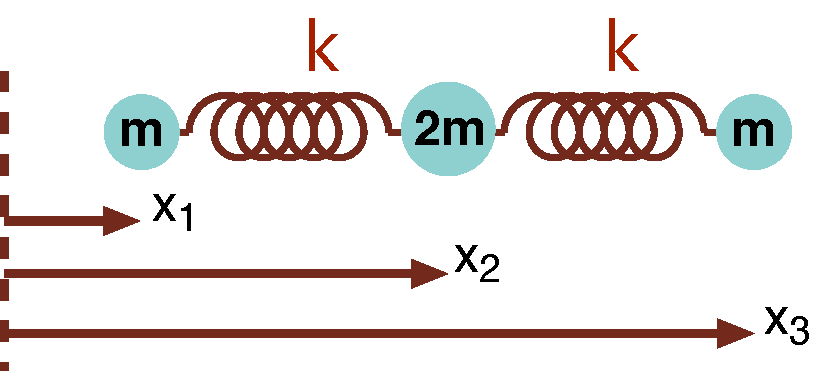
\includegraphics[width=0.5\textwidth]{figs/springs}}
\caption{\label{fig:springs} For Example
  \ref{sec:lagrangians}.\arabic{examplecounter}, three masses
  connected by two springs. The center-of-mass motion is unaffected by
  the springs.}
\end{figure}
Consider two springs, whose relaxed lengths are $\ell$, connected to
three masses as depicted in Fig. \ref{fig:springs}. Describe the two
normal modes of the motion. We can write the Lagrangian as
\begin{eqnarray*}
\mathcal{L}&=&\frac{m}{2}\dot{x}_1^2+m\dot{x}_2^2+\frac{m}{2}\dot{x}_3^2
-\frac{k}{2}(x_2-x_1-\ell)^2-\frac{k}{2}(x_3-x_2-\ell)^2.
\end{eqnarray*}
There are three coordinates, thus there are three equations of motion,
\begin{eqnarray*}
m\ddot{x}_1&=&-k(x_1-x_2+\ell)\\ 2m\ddot{x}_2&=&-k(x_2-x_1-\ell)-k(x_2-x_3+\ell)\\ &=&-k(2x_2-x_1-x_3)\\ m\ddot{x}_3&=&-k(x_3-x_2+\ell).
\end{eqnarray*}
This is a bit complicated because the center-of-mass motion does not
easily separate from the three equations. Instead, choose the
following coordinates,
\begin{eqnarray*}
X&=&\frac{x_1+2x_2+x_3}{4},\\ q_1&=&x_1-x_2+\ell,\\ q_3&=&x_3-x_2-\ell.
\end{eqnarray*}
In these coordinates the potential energy only involves two
coordinates,
\begin{eqnarray*}
U&=&\frac{k}{2}(q_1^2+q_3^2).
\end{eqnarray*}
To express the kinetic energy express $x_1, x_2$ and $x_3$ in terms of
$X$, $q_1$ and $q_3$,
\begin{eqnarray*}
x_1&=&(3q_1-q_3-4\ell+4X)/4,\\ x_2&=&(4X-q_1-q_3)/4,\\ x_3&=&(3q_3-q_1+4\ell+4X)/4.
\end{eqnarray*}
The kinetic energy and Lagrangian are them
\begin{eqnarray*}
T&=&\frac{m}{2}\frac{1}{16}(3\dot{q}_1-\dot{q}_3+4\dot{X})^2
+m\frac{1}{16}(4\dot{X}-\dot{q}_1-\dot{q}_3)^2
+\frac{m}{2}\frac{1}{16}(3\dot{q}_3-\dot{q}_1+4\dot{X})^2\\ &=&\frac{3m}{8}(\dot{q}_1^2+\dot{q}_3^2)-\frac{m}{4}\dot{q}_1\dot{q}_3
+2m\dot{X}^2,\\ \mathcal{L}&=&\frac{3m}{8}(\dot{q}_1^2+\dot{q}_3^2)-\frac{m}{4}\dot{q}_1\dot{q}_3
+2m\dot{X}^2-\frac{k}{2}q_1^2-\frac{k}{2}q_3^2.
\end{eqnarray*}
The three equations of motion are then,
\begin{eqnarray*}
\frac{3}{4}m\ddot{q}_1-\frac{1}{4}m\ddot{q}_3&=&-kq_1,\\ \frac{3}{4}m\ddot{q}_3-\frac{1}{4}m\ddot{q}_1&=&-kq_3,\\ 4M\ddot{X}&=&0.
\end{eqnarray*}
The last equation simply states that the center-of-mass velocity is
fixed. One could obtain the same result by summing the equations of
motion for $x_1$, $2x_2$ and $x_3$ above. The second two equations are
more complicated. To solve them, we assume a form
\begin{eqnarray*}
q_1&=&Ae^{i\omega t},\\ q_3&=&Be^{i\omega t},
\end{eqnarray*}
Because this is a linear equation, we can multiply the solution by a
constant and it will still be a solution. Thus, we can set $B=1$, then
solve for $A$, effectively solving for $A/B$. Putting this guess into
the equations of motion,
\begin{eqnarray*}
-\frac{3}{4}\frac{A}{B}\omega^2+\frac{1}{4}\omega^2&=&-\omega_0^2\frac{A}{B},\\ \frac{3}{4}\omega^2+\frac{1}{4}\frac{A}{B}\omega^2&=&-\omega_0^2.
\end{eqnarray*}
This is two equations and two unknowns, $\omega^2$ and
$A/B$. Substituting for $A/B$ gives a quadratic equation,
\begin{eqnarray*}
\omega^4-3\omega_0^2\omega^2+2\omega_0^4&=&0,\\ \omega_0^2&\equiv&k/m.
\end{eqnarray*}
The two solutions are
\begin{eqnarray*}
(1)~~\omega&=&\omega_0,~~~A=-B,\\ (2)~~\omega&=&\omega_0\sqrt{2},~~~A=B.
\end{eqnarray*}
The first solution corresponds to the two outer masses moving in
opposite directions, in sync, with the middle mass fixed. The second
solution has both outer masses moving in the same direction, but with
the center mass moving opposite. These two solutions are referred to
as normal modes, and are characterized by their frequency and by the
linear combinations of coordinates that oscillate together. In
general, the solution is a linear combination of normal modes, which
usually results in a chaotic looking motion. However, once the
solution is expressed in terms of the normal modes, each of which
oscillates independently in a simple manner, one can better understand
the motion. Further, the frequencies of these modes represent the
natural resonant frequencies of the system. This is important in the
construction of many structures, such as bridges or vehicles.

\example Consider a double pendulum confined to the $x-y$ plane, where
$y$ is vertical. A mass $m$ is connected to the ceiling with a
massless string of length $\ell$. A second mass $m$ hangs from the
first mass with an identical massless string of the same length. Using
$\theta_1$ and $\theta_2$ to describe the orientations of the strings
relative to the vertical axis, find the Lagrangian and derive the
equations of motion, both for arbitrary angles and in the small-angle
approximation. Finally, express the equations of motion in the limit
of small oscillations.

{\bf Solution:}\\ The kinetic and potential energies are:
\begin{eqnarray*}
T&=&\frac{1}{2}m\ell^2\dot{\theta}_1^2
+\frac{1}{2}m\left\{(\ell\dot{\theta}_1\cos\theta_1+\ell\dot{\theta}_2\cos\theta_2)^2
+(\ell\dot{\theta}_1\sin\theta_1+\ell\dot{\theta}_2\sin\theta_2)^2\right\}\\ &=&\frac{1}{2}m\ell^2\left\{2\dot{\theta}_1^2+\dot{\theta}_2^2+2\dot{\theta}_1\dot{\theta}_2\cos(\theta_1-\theta_2)
\right\},\\ U&=&mg\ell(1-\cos\theta_1)+mg\left[\ell(1-\cos\theta_1)+\ell(1-\cos\theta_2)\right]\\ &=&mg\ell(3-2\cos\theta_1-\cos\theta_2)
\end{eqnarray*}
Lagrange's equations for $\theta_1$ lead to
\begin{eqnarray*}
m\ell^2\frac{d}{dt}\left\{2\dot{\theta}_1+\dot{\theta}_2\cos(\theta_1-\theta_2)\right\}&=&
-m\ell^2\dot{\theta}_1\dot{\theta}_2\sin(\theta_1-\theta_2)
-2mg\ell\sin\theta_1,\\ 2\ddot{\theta}_1+\ddot{\theta}_2\cos(\theta_1-\theta_2)+\dot{\theta}_2^2\sin(\theta_1-\theta_2)
&=&-2\omega_0^2\sin\theta_1,\\ \omega_0^2&\equiv& g/\ell,
\end{eqnarray*}
and the equations for $\theta_2$ are
\begin{eqnarray*}
m\ell^2\frac{d}{dt}\left\{\dot{\theta}_2+\dot{\theta}_1\cos(\theta_1-\theta_2)\right\}&=&
m\ell^2\dot{\theta}_1\dot{\theta}_2\sin(\theta_1-\theta_2)-mg\ell\sin\theta_2,\\ \ddot{\theta}_2+\ddot{\theta_1}\cos(\theta_1-\theta_2)&=&
-\omega_0^2\sin\theta_2.
\end{eqnarray*}
For small oscillations, one can only consider terms linear in
$\theta_1$ and $\theta_2$ or their derivatives,
\begin{eqnarray}
\label{eq:doublependulum}
2\ddot{\theta}_1+\ddot{\theta}_2&=&-2\omega_0^2\theta_1,\\ \nonumber
\ddot{\theta}_1+\ddot{\theta}_2&=&-\omega_0^2\theta_2.
\end{eqnarray}
To find the solutions, assume they are of the form
$\theta_1=Ae^{i\omega t}, \theta_2=Be^{i\omega t}$. Solve for $\omega$
and $A/B$, noting that $B$ is arbitrary.

Plug in the desired form and find
\begin{eqnarray*}
e^{i\omega t}(-2\omega^2A-\omega^2B)&=&e^{i\omega
  t}(-2\omega_0^2A),\\ e^{i\omega
  t}(-\omega^2A-\omega^2B)&=&e^{i\omega t}(-\omega_0^2B).
\end{eqnarray*}
We can treat $B$ as arbitrary and set it to unity. When we find $A$,
it is the same as $A/B$ for arbitrary $B$. This gives the equations
\begin{eqnarray*}
2\omega^2A+\omega^2&=&2\omega_0^2A,\\ \omega^2A+\omega^2&=&\omega_0^2.
\end{eqnarray*}
This is two equations and two unknowns. Solving them leads to a
quadratic equation with solutions
\begin{eqnarray*}
A/B&=&\pm\frac{1}{\sqrt{2}},\\ \omega^2&=&\frac{\omega_0^2}{1\pm
  1/\sqrt{2}}.
\end{eqnarray*}
Again, these two solutions are the normal modes, and the general
solution is a sum of the two solutions, with two arbitrary
constants. For the angles $\theta_1$ and $\theta_2$ are:
\begin{eqnarray*}
\theta_1&=&\frac{A_+}{\sqrt{2}}e^{i\omega_+t},
~\theta_2=A_+e^{i\omega_+t},\\ \theta_1&=&\frac{-A_-}{\sqrt{2}}e^{i\omega_-t},
~\theta_2=A_-e^{i\omega_-t},\\ \omega_{\pm}&=&\omega_0\sqrt{\frac{1}{1\pm
    1/\sqrt{2}}}.
\end{eqnarray*}
One can also express the solution in vector notation, with the vectors
having arbitrary amplitudes $A_+$ and $A_-$,
\begin{eqnarray*}
\theta_+&=&\left(\begin{array}{c}
  \frac{1}{\sqrt{2}}\\ 1\end{array}\right)A_+e^{i\omega_+t},\\ \theta_-&=&\left(\begin{array}{c}
    \frac{-1}{\sqrt{2}}\\ 1\end{array}\right)A_-e^{i\omega_-t}.
\end{eqnarray*}
Here, the upper/lower components of the vector describe
$\theta_1/\theta_2$ respectively.

\exampleend

{\bf Aside:} (not applied in this course)\\ These problems can be
treated as linear algebra exercises. Linear algebra is not used in
this course, but nonetheless we describe how this works for the
curious student. In the limit of small vibrations, the equations of
motion can be expressed in the form,
\begin{eqnarray*}
M\ddot{q}&=&-Kq,
\end{eqnarray*}
a form that looks like the spring equation. However, $q$ is an
$n-$dimensional vector and $M$ and $k$ are $n\times n$ matrices. In
the double pendulum example, the dimensionality is 2 and the $q$
refers to the $\theta_1$ and $\theta_2$, and the matrices for $M$ and
$K$ can be read off Eq. (\ref{eq:doublependulum}),
\begin{eqnarray*}
M&=&\left(\begin{array}{cc}
  2&1\\ 1&1\end{array}\right)~,\hspace*{40pt}
  K=\left(\begin{array}{cc}
    2\omega_0^2&0\\ 0&\omega_0^2\end{array}\right).
\end{eqnarray*}
Multiplying both sides of the equation by the inverse matrix $M^{-1}$,
\begin{eqnarray*}
\ddot{q}&=&-\left(M^{-1}K\right)q.
\end{eqnarray*}
Here,
\begin{eqnarray*}
M^{-1}&=&\left(\begin{array}{cc}
  1&-1\\ -1&2\end{array}\right),\\ M^{-1}K&=&\left(\begin{array}{cc}
    2&-1\\ -2&2\end{array}\right)\omega_0^2.
\end{eqnarray*}
One can find a transformation, basically a rotation, that transforms
to a frame where $M^{-1}K$ is diagonal. In this coordinate system the
diagonal components of $M^{-1}K$ represent the squared frequencies of
the normal modes,
\[
M^{-1}K\rightarrow -\left(\begin{array}{cc}
  \omega_+^2&0\\ 0&\omega_-^2\end{array}\right)~,
\]
and are known as ``eigen'' frequencies. The corresponding unit
vectors,
\[
\left(\begin{array}{c} 1\\0\end{array}\right)~{\rm
    and}~\left(\begin{array}{c} 0\\1\end{array}\right)~{\rm
      in~the~new~coordinate~system},
\]
can be rotated back into the original frame, and become the solutions
for the normal modes. These are then called ``eigenvectors'', which
are the same as the normal modes. Finding the eigenfrequencies is
performed by realizing that the determinant of a matrix is unchanged
by the rotation between coordinate systems. Writing the equations of
motion as an eigenvalue problem,
\begin{eqnarray}
\left[A-\lambda_i\mathbb{1}\right]u_i&=&0,~~~A\equiv
M^{-1}K,~\lambda_i\equiv \omega^2_i.
\end{eqnarray}
In the coordinate system where $M^{-1}K$ is diagonal, and the forms
for $u_i$ are simple this requires that in that system, the diagonal
elements of $M^{-1}K$ are the eigenvalues, $\omega_i^2$. For each
$\omega^2_i$, the determinant $|A-\lambda_i\mathbb{1}|$ must
vanish. This is then true in any coordinate system,
\begin{eqnarray}
{\rm det}\left[A-\lambda\mathbb{1}\right]&=&0,
\end{eqnarray}
which for a $2\times 2$ matrix becomes
\begin{eqnarray}
\label{eq:eigen}
\left|
\begin{array}{cc}
A_{11}-\lambda&A_{12}\\ A_{21}&A_{22}-\lambda
\end{array}
\right|&=&0,\\ A_{11}A_{22}-\lambda A_{11}-\lambda
A_{22}+\lambda^2-A_{21}A_{12}&=&0.
\end{eqnarray}
One can solve a quadratic equation for $\lambda$, which gives two
eigenvalues corresponding to $\omega_+^2$ and $\omega_-^2$ found
above. Choosing one of the eigenvalues, one can insert one of the
eigenvalues $\lambda_i$ into Eq. (\ref{eq:eigen}) and solve for $u_i$,
then choose the other eigenvalue and solve for the other corresponding
vector.

If this were a 3-dimensional set of equations, the determinant would
include terms like $\lambda^3$ and would become a cubic equation with
three eigenvalues. One would then solve for three eigenvectors. If one
has a system with dimensionality $n>2$, one usually resorts to solving
the problem numerically due to the messiness of the algebra. The main
programming languages all have packages which readily diagonalize
matrices and find eigenvectors and eigenvalues.
\subsection{Conservation Laws}

Energy is conserved only when the Lagrangian has no explicit
dependence on time, i.e. $L(q,\dot{q})$, not $L(q,\dot{q},t)$. To show
this, we first define the Hamiltonian,
\begin{eqnarray}
\label{eq:Hdef}
H&=&\sum_i\left(\dot{q}_i\frac{\partial
  L}{\partial\dot{q}_i}\right)-L.
\end{eqnarray}
After showing that $H$ is conserved, i.e. $(d/dt)H=0$, we then show
that $H$ can be identified with the total energy, $H=T+V$.

One can see that $H$ is conserved by applying first using the chain
rule for $(d/dt)H$ in Eq. (\ref{eq:Hdef}), then applying Lagrange's
equations,
\begin{eqnarray}
\frac{d}{dt}H&=&\sum_i\left\{\ddot{q}_i\frac{\partial
  L}{\partial\dot{q}_i}+\dot{q}_i\frac{d}{dt}\left(\frac{\partial
  L}{\partial\dot{q}_i}\right)-\frac{\partial
  L}{\partial\dot{q}_i}\ddot{q}_i-\frac{\partial L}{\partial
  q_i}\dot{q}_i\right\}\\ \nonumber
&=&\sum_i\left\{\ddot{q}_i\frac{\partial
  L}{\partial\dot{q}_i}+\dot{q}_i\frac{\partial L}{\partial
  q_i}-\frac{\partial L}{\partial\dot{q}_i}\ddot{q}_i-\frac{\partial
  L}{\partial q_i}\dot{q}_i\right\}\\ \nonumber &=&0.
\end{eqnarray}
These steps assumed that $L$ had no explicit time dependence, i.e. $L$
is a function of $q$ and $\dot{q}$, but not of $t$.

Next, we show that $L$ can be identified with the energy. Because $V$
does not depend on $\dot{q}$,
\begin{equation}
H=\sum_i\frac{\partial T}{\partial\dot{q}_i}\dot{q}_i-T+V.
\end{equation}
If the kinetic energy has a purely quadratic form in terms of
$\dot{q}$,
\begin{equation}
\label{eq:Hquadq}
T=\sum_{ij}A_{ij}(q)\dot{q}_i\dot{q}_j,
\end{equation}
the Hamiltonian becomes
\begin{eqnarray}
H&=&\sum_{ij}2A_{ij}(q)\dot{q}_i\dot{q}_j-\sum_{ij}A_{ij}(q)\dot{q}_i\dot{q}_j+V\\ \nonumber
&=&T+V.
\end{eqnarray}
The proof that $H$ equals the energy hinged on the fact that the
kinetic energy was quadratic in $\dot{q}$. This can be attributed to
time-reversal symmetry. Because the Cartesian coordinates $x_i$ do not
depend on $\dot{q}_i$ or on time, $\dot{x}_i=(\partial x_i/\partial
q_j)\dot{q}_j$. Thus, the kinetic energy, $T=m\dot{x}_i^2/2$, should
be proportional to two powers of $\dot{q}$, which validates the
assumption in Eq. (\ref{eq:Hquadq}).

Here, energy conservation is predicated on the Lagrangian not having
an explicit time dependence. Without an explicit time dependence the
equations of motion are unchanged if one translates a fixed amount in
time because the physics does not depend on when the clock starts. In
contrast, the absolute time becomes relevant if there is an explicit
time dependence. In fact, conservation laws can usually be associated
with symmetries. In this case the translation symmetry in time leads
to energy conservation.

For another example of how symmetry leads to conservation laws,
consider a Lagrangian for a particle of mass $m$ moving in a
two-dimensional plane where the generalized coordinates are the radius
$r$ and the angle $\theta$. The kinetic energy would be
\begin{equation}
T=\frac{1}{2}m\left\{\dot{r}^2+r^2\dot{\theta}^2\right\},
\end{equation}
and if the potential energy $V(r)$ depends only on the radius $r$ and
not on the angle, Lagrange's equations become
\begin{eqnarray}
\frac{d}{dt}(m\dot{r})&=&-\frac{\partial V}{\partial
  r}+m\dot{\theta}^2r,\\ \nonumber \frac{d}{dt}(mr^2\dot{\theta})&=&0.
\end{eqnarray}
The second equation implies that $mr^2\dot{\theta}$ is a
constant. Indeed, it is the angular momentum which is conserved for a
radial force. Here, the conservation of angular momentum is associated
with the independence of the physics to changes in $\theta$, or in
other words, rotational invariance. Once one knows the fact that
$L=mr^2\dot{\theta}$ is conserved, it can be inserted into the
equations of motion for $\dot{r}$,
\begin{equation}
m\ddot{r}=-\frac{\partial V}{\partial r}+\frac{L^2}{mr^3}.
\end{equation}
This is related to Noether's theorem
\href{http://en.wikipedia.org/wiki/Noether's_theorem}{http://en.wikipedia.org/wiki/Noether's\_theorem},
named after Emmy Noether,
\href{http://en.wikipedia.org/wiki/Emmy_Noether}{http://en.wikipedia.org/wiki/Emmy\_Noether}. Simply
stated, if the Lagrangian $L$ is independent of $q_i$, one can see
that the quantity $\partial L/\partial\dot{q}_i$ is conserved,
\begin{equation}
\label{eq:noether}
\frac{d}{dt}\frac{\partial L}{\partial\dot{q}_i}=0.
\end{equation}

Another easy example is in Cartesian coordinates where the potential
depends only on $x$ and $y$ but not on $z$. In that case, there is a
translational symmetry. From Eq. (\ref{eq:noether}), this translates
into conservation of the momentum in the $z$ direction.

\example Consider a pair of particles of mass $m_1$ and $m_2$ where
the potential is of the form
\[
U(\vec{r}_1,\vec{r}_2)=V_a(|m_1\vec{r}_1+m_2\vec{r}_2|/(m_1+m_2))+V_b(|\vec{r}_1-\vec{r}_2|).
\]
Using symmetry arguments alone, are there any conserved components of
the momentum? or the angular momentum??\\

There is no translational invariance, hence there are no conserved
components of the momentum. However, there is rotational invariance
about any axis that goes through the origin. Hence, there is angular
momentum conservation in all three directions. Symmetry arguments are
great ways to recognize the existence of conserved quantities, but
actually expressing them in terms of coordinates can be tricky. For
instance, you may need to write the Lagrangian in terms of angles.

\exampleend

\subsection{Numerically Solving Differential Equations}

Lagrangians lead to equations of motion for the generalized
coordinates. Often, these equations are not analytically solvable, but
are readily addressed computationally. Here, we demonstrate how one
would solve such an equation numerically. So, we first imagine we have
a differential equation for $y(t)$, and for this example we assume the
equation has no derivatives higher than second order. If the boundary
conditions fix $y(0)$ and $y'(0)$, this should be sufficient to
determine $y(t)$ for all future times. Of course, computers need to
discretize the time steps. So assume there are time steps separated by
$\Delta t$ and values,
\begin{eqnarray}
t_n&=&n\Delta t,~=0,\Delta t, 2\Delta t, 3\Delta t\cdots\\ \nonumber
y_n&=&y(t_n).
\end{eqnarray}
Our first step is to solve for $y_{-1}$ and $y_1$ given $y_0$ and
$y'_0$. Approximating the derivatives over the finite intervals,
\begin{eqnarray}
y(0)&=&y_0,\\ \nonumber y'(0)&=&\frac{y_1-y_{-1}}{2\Delta
  t},\\ \nonumber y''(0)&=&\frac{1}{\Delta
  t}\left\{\frac{y_1-y_0}{\Delta t}-\frac{y_0-y_{-1}}{\Delta
  t}\right\} =\frac{y_1-2y_0+y_{-1}}{\Delta t^2}.
\end{eqnarray}
One needs to solve for the three unknowns $y_{-1},y_0$ and
$y_1$. Here, $y(0)$ and $y'(0)$ are given, but $y''(0)$ is not, so a
third equation is needed to solve for the three unknowns. This is
provided by the equations of motion from the Lagrangian. Solving 3
equations and 3 unknowns is thus a fair fight, and one can determine
$y_{-1}\rightarrow y_1$. Once knows these three values, one can use
the differential equation to solve for $y_2$ using $y_0$ and
$y_1$. One can then iteratively find $y_n$ for any $n$ given $y_{n-1}$
and $y_{n-2}$.

\example

Write an algorithm for solving the driven harmonic oscillator,
\[
y''(t)+2\beta y'(t)+\omega_0^2 y(t)=(F_0/m)\cos\omega t.
\]
given $y'(0)=6$ m/s, $y(0)=0.3$ m, and given $m=0.5$ kg, $F_0=400$ N,
and a spring constant $k=2000$ N/m. Let the driving force have a
period of 2.5 s, and the damping rate be $\beta=0.15$ s$^{-1}$.

Let's first solve for $y$ with indices $a,b,c=-1,0,1$, using the
differential equation and the boundary conditions. The BC state that
$y_b=0.3$ m and $(y_c-y_a)=2\Delta t y'_b$, where $y'_b=6$
m/s. Writing the differential equation,
\begin{eqnarray*}
\frac{y_c-2y_b+y_a}{\Delta t^2}+\beta\frac{y_c-y_a}{\Delta
  t}+\omega_0^2 y_b&=&(F_0/m)\cos\omega t_b,
\end{eqnarray*}
one can substitute for $y_a$ because the boundary condition for
$y'_b=y'_0$ gives $y_a=y_{-1}$,
\begin{eqnarray*}
y_a&=&y_c-2\Delta ty'_b,
\end{eqnarray*}
which gives an equation for $y_c$, where everything else in known,
\begin{eqnarray*}
\frac{2y_c-2y_b-2y'_b\Delta t}{\Delta t^2}+2\beta
y'_b+\omega_0^2y_b&=&f_b,\\ \nonumber y_c&=&y_b+y'_b\Delta
t+\left[(f_b/2)-(\omega_0^2y_b/2)-\beta y'_b\right](\Delta t)^2.
\end{eqnarray*}
Here, $f_b\equiv (F_0/m)\cos\omega t$.

Now, that one knows $y_0$ and $y_1$, lets write the differential
equation for three consecutive points $y_a$, $y_b$ and $y_c$, and
solve for $y_c$ in terms of the other two (rather than using the BC as
was done above). Again, beginning with the differential equation,
\begin{eqnarray*}
\frac{y_c-2y_b+y_a}{\Delta t^2}+\beta\frac{y_c-y_a}{\Delta
  t}+\omega_0^2 y_b&=&(F_0/m)\cos\omega
t_b,\\ y_c\left(\frac{1}{\Delta t^2}+\frac{\beta}{\Delta t}\right)
&=&f_b-\omega_0^2y_b+\frac{2y_b-y_a}{\Delta t^2}+\frac{\beta
  y_b}{\Delta
  t},\\ y_c&=&\frac{f_b-\omega_0^2y_b+\frac{2y_b-y_a}{\Delta
    t^2}+\frac{\beta y_b}{\Delta t}}{\frac{1}{\Delta
    t^2}+\frac{\beta}{\Delta t}},\\ &=&\frac{f_b\Delta
  t^2-\omega_0^2y_b\Delta t^2+2y_b-y_a+\beta y_b\Delta
  t}{1+\beta\Delta t}.
\end{eqnarray*}
Using $a=0, b=1, c=2$, this gives $y_2$. Then one can repeat with
$a=1, b=2$ and $c=3$ to find $y_3$, and iterate to find all $n$.

{\bf Solution}:\\ The code might look something like this:
{\tt \begin{verbatim} void main(){ const double PI=4.0*atan(1.0);
    double m=0.5,k=2000.0; double omega0=sqrt(k/m), omega=2.0*PI/2.5,
    beta=0.15; double ya,yb,yc,Dt=0.0025; // Dt = Delta t double
    F0=400,yprime0; // Solve for a,b,c=-1,0,1, solve for yc yb=0.3;
    yprime0=6.0; fb=(F0/m); // Use BC to solve for y_1=yc, from
    lecture notes yc=yb+yprime0*Dt
    +(0.5*fb-0.5*omega0*omega0*yb-beta*yprime0)*Dt*Dt; printf("t=0,
    y=%g\n",yb);
   
   // Now interatively solve for yc, beginning with yc=y_2
   for(n=0;n<1000;n++){ ya=yb; yb=yc; t=(n+1)*Dt;
     fb=(F0/m)*cos(omega*t);
     yc=(fb*Dt^2-omega0^2*yb*Dt*Dt+2*yb-ya+beta*yb*Dt)/(1+beta*Dt);
     printf("t=%g, y=%g\n",Dt*n,yb); } }
\end{verbatim}}
\hrulefill

\subsection{Exercises}

\begin{enumerate}

\item Consider a hill whose height $y$ is given as a function of the
  horizontal coordinate $x$. Consider a segment of the hill from $x=0$
  to $x=L$ with initial height $y(x=0)=0$ and whose final height is
  $y(x=L)=-h$. Transforming the last equation in Example
  \ref{ex:brachiostone} for a downward vertical force rather than a
  horizontal force,
\[
x=-\sqrt{-2ay-y^2}+a\arccos(1+y/a).
\]
Consider a wheel of radius $a$ rolling along the bottom of the $x$
axis. Mark a point on the top of the wheel, which is originally at the
origin, $x=y=0$, when the top of the wheel touches the origin. As the
wheel rolls by an angle $\theta$ the marked point moves due to both
the translation and the rotation of the wheel. The $y$ coordinate of
the marked point is
\[
y=-a(1-\cos\theta),
\]
whereas the $x$ coordinate is
\[
x=a\theta-a\sin\theta.
\]
The first term is due to the horizontal translation of the axis, while
the second term arises from the rotation of the wheel. Re-express
these two equations to find $x(y)$.

\item Consider a chain of length $L$ that hangs from two supports of
  equal height stretched from $x=-X$ to $x=+X$. The general solution
  for a catenary is
\[
y=\lambda+a\cosh[(x-x_0)/a],
\]
\begin{enumerate}
\item Using symmetry arguments, what is $x_0$?
\item Express the length $L$ in terms of $X$ and $a$.
\item Numerically solve the transcendental equation above to find $a$
  in terms of $L=10$ m and $X=4$ m.
\end{enumerate}

\item Consider a mass $m$ connected to a spring with spring constant
  $k$. Rather than being fixed, the other end of the spring oscillates
  with frequency $\omega$ and amplitude $A$. For a generalized
  coordinate, use the displacement of the mass from its relaxed
  position and call it $y=x-\ell-A\cos\omega t$. In this system the
  potential energy of the spring is $ky^2/2$.
\begin{enumerate}
\item Write the kinetic energy in terms of the generalized coordinate.
\item Write down the Lagrangian.
\item Find the equations of motion for $y$.
\end{enumerate}

\item Consider a bead of mass $m$ on a circular wire of radius
  $R$. Assume a force $kx$ acts on the bead, where $x$ and $y$ axes
  run through the center of the circle. Using $\theta$ as the
  generalized coordinate (measured relative to the $x$ axis),
\begin{enumerate}
\item Write the Lagrangian in terms of $\theta$.
\item Find the equations of motion.
\end{enumerate}

\item Consider a pendulum of length $\ell$ with all the mass $m$ at
  its end. The pendulum is allowed to swing freely in both
  directions. Using $\phi$ to describe the azimuthal angle about the
  $z$ axis and $\theta$ to measure the angular deviation of the
  pendulum from the downward direction, address the following
  questions:
\begin{enumerate}
\item If the pendulum is initially moving horizontally with velocity
  $v_0$ and angle $\theta_0=90^\circ$ (horizontal), use energy and
  angular momentum conservation to find the minimum angles of
  $\theta_{\rm min}$ subtended by the pendulum. (Note that the angle
  will oscillate between $90^\circ$ and the minimum angle.
\item Write the Lagrangian using $\theta$ and $\phi$ as generalized
  coordinates.
\item Write the equations of motion for $\theta$ and $\phi$.
\item Rewrite the equations of motion for $\theta$ using angular
  momentum conservation to eliminate and reference to $\phi$.
\item Find the value of $L$ required for the stable orbit to be at
  $\theta=45^\circ$.
\item For the steady orbit found in (e) consider small perturbations
  of the orbit. Find the frequency with which the pendulum oscillates
  around $\theta=45^\circ$.
\end{enumerate}

\item Consider a mass $m$ that is connected to a wall by a spring with
  spring constant $k$. A second identical mass $m$ is connected to the
  first mass by an identical spring. Motion is confined to the $x$
  direction.
\begin{enumerate}
\item Write the Lagrangian in terms of the positions of the two masses
  $x_1$ and $x_2$.
\item Solve for the equations of motion.
\item Find two solutions of the type
\begin{eqnarray*}
x_1&=&Ae^{i\omega t},~~~x_2=Be^{i\omega t}.
\end{eqnarray*}
Solve for $A/B$ and $\omega$. Express your answers in terms of
$\omega_0^2=k/m$.
\end{enumerate}

\item Consider two masses $m_1$ and $m_2$ interacting according to a
  potential $V(\vec{r}_1-\vec{r}_2)$.
\begin{enumerate}
\item Write the Lagrangian in terms of the generalized coordinates
  $\vec{R}_{\rm cm}=(m_1\vec{r}_1+m_2\vec{r}_2)/(m_1+m_2)$ and
  $\vec{r}=\vec{r}_1-\vec{r}_2$, and their derivatives.
\item Using the independence of the Lagrangian with respect to
  $\vec{R}_{\rm cm}$, find expressions for the conserved total
  momentum.
\end{enumerate}

\end{enumerate}
%\end{document}
